\documentclass[twocolumn]{article}
\usepackage{hyperref}
\usepackage{titling}
\usepackage{graphicx}

\DeclareGraphicsExtensions{.png}

\setlength{\droptitle}{-10em}

%opening
\title{User Error}
\author{Success is the absence of error}
\date{}

\begin{document}

\maketitle

\section*{Authors}

\emph{User Error} was created by Jeremy Vasta, Sam Bloomberg, Liam Middlebrook, Alex Harper, Oliver Barnum, and Alex Hoshino.

\section*{Premise}

Welcome to your job as a manager for an outsourced IT firm! You are going to be competing against other firms for the satisfaction of our company. Careful, though, if things get too chaotic the entire company might go under!

\section*{Materials}

\begin{itemize}
	\item Asset Deck (Equipment and Technicians)
	\item Issue Deck (Issues)
	\item Business Deck (Audits and Contracts)
	\item Stability sheet
	\item Stability marker
	\item 4 $\times$ satisfaction sheets
	\item 4 $\times$ satisfaction markers
	\item 6-sided die
	\item First player marker
	\item Budget counters
\end{itemize}

\section*{Setup}

Start by separating out the business deck, the asset deck, and the issue deck. Find the "end of game" card (it is a business card) and put it aside. Shuffle the three decks separately. Shuffle the "end of game" card into the last 5 cards of the business deck. Place each deck on the table. Place the stability/turn sheet in the center where all players can see it, and place the turn and stability markers at the beginning of their respective tracks.

Each player receives a satisfaction sheet, and places a satisfaction marker at the 0 position on their sheet. Each player also receives 3 budget counters.

The first player marker starts with whomever last called IT or tech support.

\subsection*{Draft}

Deal a number of asset cards face up on the table equal to 2 $\times$ the number of players. Players take turns starting with the first player and continuing in a counter-clockwise direction, buying a single asset at a time. This continues until no one wants to or is able to buy any more assets. Players are not forced to buy assets, though it is in their best interest to do so.

Once initial acquisition is completed, all remaining asset cards are shuffled back into the asset deck. \newline

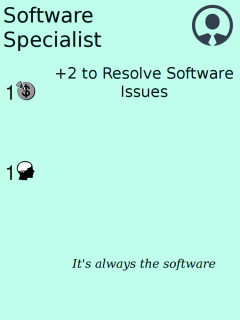
\includegraphics{asset_example}
\newline
\small{Asset Card}

\section*{Winning and Losing}

If at any time the stability marker is at or past the last space on the stability track, all players lose regardless of their satisfaction and the company goes under due to the chaos. Barring that, the game ends when the "end of game" card is played from the business deck, with the player that has the highest customer satisfaction winning.

Satisfaction is gained by completing issues each turn, and is lost by having issues that are incomplete at the end of your turn.

\section*{Phases}

Once initial acquisition is completed, play continues with the following phases for the rest of the game: \emph{Dispatch}, \emph{Troubleshooting}, \emph{Negotiation}, and \emph{Evaluation}.

\subsection*{Dispatch}

Players are dealt a number of issues corresponding to the current row the stability marker is at into their backlog (their hand). Players may assign at most one issue per technician. Issues should stay visible to all players, even if in a backlog. \newline

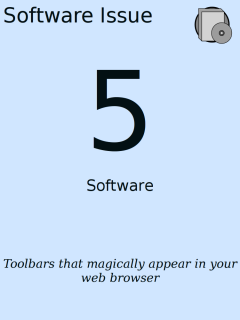
\includegraphics[scale=1]{issue_example}
\newline
\small{Issue Card}

\subsection*{Troubleshooting}

Players take turns (starting with the first player, and proceeding in a clockwise direction) either
resolving or referring a single issue that is assigned to a technician. This phase ends once actions have been taken for all assigned issues.

\subsubsection*{Resolving Issues}

To resolve an issue, announce which issue/technician you are attempting to resolve (you can not re-assign an issue to a different technician in the same turn). Roll the D6 and add the technician's skill to the value on the die. If the technician, or any equipment you may have, gives a bonus to the type of issue you are trying to resolve, add that as well. If the total is equal to or greater than the difficulty of the issue, the issue is resolved, discarded, and you may move your satisfaction marker up by one.
If you fail to resolve the issue, it is returned to your backlog.

\subsubsection*{User Errors}

User errors cannot be resolved except by cards with relevant abilities.

\subsubsection*{Referring Issues}

If an issue has a difficulty that exceeds your technician's skill by at least 4 or if the issue is a \emph{User Error}, you may put the issue into any other player's backlog. That issue may not be further resolved or referred until the next troubleshooting phase.


\subsection*{Negotiation}

A single contract card is dealt face-up on the table. Players hide a number of budget counters equal to or lower than the budget value on the contract in their hand. Once all players are ready, reveal the amount of budget in your hand. The player who bid the lowest amount gets the contract and the associated budget.

Players may not bid on contracts that have the same effect as contracts the player already has, unless said contracts have been abandoned.

If a player does not want to bid, they must announce it before bidding commences. Bidding no budget is still a valid bid.

If there is a tie, the player with the least contracts wins the bidding. If there is still a tie, a dice roll breaks the tie.

This phase happens twice, but a player may only win a contract once. \newline

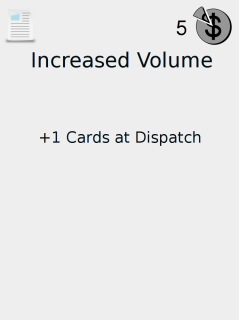
\includegraphics{business_example}
\newline
\small{Business Card}

\subsubsection*{Audits}

If either contract that was dealt is an \emph{Audit} card, then an audit occurs. All abandoned contracts must be discarded and players who had those contracts lose any budget associated with them, firing any assets to make up for that loss of budget. Any assets that have \emph{audit risk} written on them are automatically fired as well, with the owning player gaining whatever budget those assets were worth. Each player will lose CSat in parallel with the number of cards lost during the audit.

Once the audit is complete, the audit is discarded and a new contract is dealt to replace it. If multiple audits are dealt in the same negotiation phase, the subsequent audits are simply discarded and replaced until there are no audits in play.

\subsubsection*{End of Game}

If the "end of game" card comes up during this phase, gameplay ends and the player with the highest customer satisfaction wins.

\subsection*{Non-contracts}

If a non-contract is drawn and discarded, replace it with another card from the business deck. This includes audits, records losses, and other non-contracts.

\subsection*{Acquisition}

A number of asset cards equal to the number of players are dealt face-up onto the table. Players take turns purchasing assets with unused budget starting with the first player and continuing clockwise. Once an asset is purchased, another asset should be dealt onto the table to replace it. This phase continues until there are no more players willing to purchase assets. At the end of the phase, all remaining assets are discarded.

\subsection*{Evaluation}

Each player loses satisfaction equal to the number of issues in their backlog. If any player is at full negative satisfaction, then the stability marker is moved a single space.

The total number of issues in all players' backlogs is totaled, excluding user errors. The stability marker is moved one space for every four issues in each player's backlog.

Once the evaluation phase ends, the first player marker is moved to the next player in the clockwise direction, and the turn marker is moved one space. If it is the tenth turn, then the player with the highest satisfaction wins. Otherwise, the game continues with the dispatch phase once again.

\section*{Firing Assets}

During the evaluation phase, a player may decide to fire one of their assets. Doing so puts the asset in the discard pile and returns any budget used to buy that asset to the player.

If at any time a player loses budget, they must fire enough assets to make up for that lost provided they don't have enough unspent budget to make up for the loss.

\section*{Abandoning Contracts}

At any time during their turn, a player may choose to abandon a contract. Doing so allows the player to keep any budget associated with a contract while also ignoring any effects of the contract. The player should flip the contract face-down to signal that it is abandoned. Abandoned contracts cannot be un-abandoned.

If a "records loss" comes up, you may recover any abandoned contracts, even if they are the same as contracts that you have not abandoned.

\section*{Running out of cards}

If at any time any of the decks are out of cards, the associated discard pile should be shuffled and used as the deck.

\section*{Phase Quick Reference}

\begin{enumerate}
	\item Dispatch
	\item Troubleshooting
	\item Negotiation
	\item Acquisition
	\item Evaluation
\end{enumerate}

\section*{License}

This document and any related materials are released under the Creative Commons BY-SA 3.0 US license. A human readable summary and the full text for this license may be found at \url{https://creativecommons.org/licenses/by-sa/3.0/us/}.

\end{document}
